%%%%%%%%%%%%%%%%%%%%%%%%%%%%%%%%%%%%%%%%%
% Beamer Presentation
% LaTeX Template
% Version 1.0 (10/11/12)
%
% This template has been downloaded from:
% http://www.LaTeXTemplates.com
%
% License:
% CC BY-NC-SA 3.0 (http://creativecommons.org/licenses/by-nc-sa/3.0/)
%
%%%%%%%%%%%%%%%%%%%%%%%%%%%%%%%%%%%%%%%%%

%----------------------------------------------------------------------------------------
%	PACKAGES AND THEMES
%----------------------------------------------------------------------------------------

\documentclass{beamer}

\mode<presentation> {

% The Beamer class comes with a number of default slide themes
% which change the colors and layouts of slides. Below this is a list
% of all the themes, uncomment each in turn to see what they look like.

%\usetheme{default}
%\usetheme{AnnArbor}
%\usetheme{Antibes}
%\usetheme{Bergen}
%\usetheme{Berkeley}
%\usetheme{Berlin}
%\usetheme{Boadilla}
%\usetheme{CambridgeUS}
\usetheme{Copenhagen}
%\usetheme{Darmstadt}
%\usetheme{Dresden}
%\usetheme{Frankfurt}
%\usetheme{Goettingen}
%\usetheme{Hannover}
%\usetheme{Ilmenau}
%\usetheme{JuanLesPins}
%\usetheme{Luebeck}
%\usetheme{Madrid}
%\usetheme{Malmoe}
%\usetheme{Marburg}
%\usetheme{Montpellier}
%\usetheme{PaloAlto}
%\usetheme{Pittsburgh}
%\usetheme{Rochester}
%\usetheme{Singapore}
%\usetheme{Szeged}
%\usetheme{Warsaw}

% As well as themes, the Beamer class has a number of color themes
% for any slide theme. Uncomment each of these in turn to see how it
% changes the colors of your current slide theme.

%\usecolortheme{albatross}
%\usecolortheme{beaver}
%\usecolortheme{beetle}
%\usecolortheme{crane}
%\usecolortheme{dolphin}
%\usecolortheme{dove}
%\usecolortheme{fly}
%\usecolortheme{lily}
%\usecolortheme{orchid}
%\usecolortheme{rose}
%\usecolortheme{seagull}
%\usecolortheme{seahorse}
%\usecolortheme{whale}
%\usecolortheme{wolverine}

%\setbeamertemplate{footline} % To remove the footer line in all slides uncomment this line
%\setbeamertemplate{footline}[page number] % To replace the footer line in all slides with a simple slide count uncomment this line

%\setbeamertemplate{navigation symbols}{} % To remove the navigation symbols from the bottom of all slides uncomment this line
}

\usepackage{graphicx} % Allows including images
\usepackage{booktabs} % Allows the use of \toprule, \midrule and \bottomrule in tables
\usepackage{animate}
%----------------------------------------------------------------------------------------
%	TITLE PAGE
%----------------------------------------------------------------------------------------

\title[Short title]{Volume estimation via integrating on a curve fitted point cloud} % The short title appears at the bottom of every slide, the full title is only on the title page

\author{\textbf{HiPEDS 2018 Cohort:} G. Bisbas, L. Castiglione, D. Grumberg, S. Karolčík, L. Keeble, D. Kulon, B. Kwan, C. McMeel, R. Miles, J. Ortiz, N. Perez-Nieves, V. Pham Ngoc, J. Vandebon, D. Vink} % Your name
\institute[Imperial College London] % Your institution as it will appear on the bottom of every slide, may be shorthand to save space
{ Imperial College London \\ % Your institution for the title page
\medskip % Your email address
}
\date{\today} % Date, can be changed to a custom date


\begin{document}

\begin{frame}
\titlepage % Print the title page as the first slide
\end{frame}



%% --------------T--H--E--O--R--Y-------------------------------------------

\begin{frame}
\frametitle{Overall structure}

\begin{itemize}
	\item  
	\item 
	\item 
	\item 
	

	
	
\end{itemize}

\end{frame}


\begin{frame}
\frametitle{The problem and the goal} 

\begin{itemize}
	\item
	
	\item 
	
\end{itemize}

\end{frame}






\begin{frame}
\frametitle{The hardware} % Table of contents slide, comment this block out to remove it
%\tableofcontents % Throughout your presentation, if you choose to use \section{} and \subsection{} commands, these will automatically be printed on this slide as an overview of your presentation

%----------------------------------------------------------------------------------------
%	PRESENTATION SLIDES
%----------------------------------------------------------------------------------------

%------------------------------------------------
 % Sections can be created in order to organize your presentation into discrete blocks, all sections and subsections are automatically printed in the table of contents as an overview of the talk
%------------------------------------------------
\begin{figure}	
	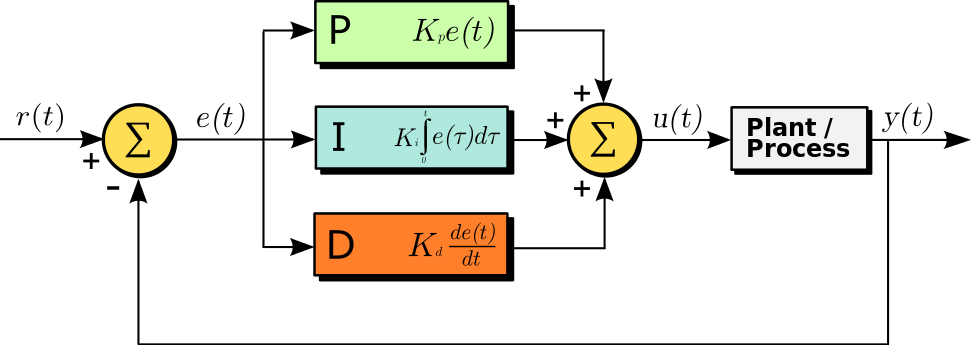
\includegraphics[width=0.8\textwidth]{Figures/PID.png}
	\caption{PID controller}
	\label{pid}
\end{figure}

\begin{itemize}
	\item

	\item 
	
\end{itemize}

\end{frame}
%\subsection{Subsection Example} % A subsection can be created just before a set of slides with a common theme to further break down your presentation into chunks

\begin{frame}\frametitle{Extracting the point cloud}



\begin{itemize}
	\item 
	\item  
	\item 
\end{itemize}


\end{frame}

\begin{frame}{PID tuning}
Adjustment of its control parameters (gain/proportional band, integral gain/reset, derivative gain/rate) to optimum values for a target response. Tuning is part of loop design, usually required if the system oscillates too much, responds too slowly, has steady-state error, or is unstable.\\
Another is known as the Ziegler-Nichols method, introduced by John G. Ziegler and Nathaniel B. Nichols of Taylor Instruments in 1942. This technique also involves setting I and D gains to zero and then increasing P gain until the loop output starts to oscillate. \\
In fact, most industrial facilities no longer tune loops with manual calculation, but use tuning and loop optimization software.  The only drawbacks: Software is somewhat costly and involves some training.\\
The analytical approach involves mathematics. \\
One can also tune by feel, which is an online method that doesn't require math. The main problem with this method is that it is erratic, not repeatable, and can be inefficient.\\
\end{frame}


\begin{frame}{PID tuning}
The final method of tuning is a quality process model called the Cohen-Coon, which is a modified version of the Ziegler-Nichols approach. This offline method involves some math, but is only good for the first-order process.

We can use this:
https://www.machinedesign.com/sensors/introduction-pid-control


\end{frame}



\begin{frame}{Embedded PID Animation}
  \animategraphics[loop,controls,width=\linewidth]{30}{Figures/PID_animated-}{1}{248}
\end{frame}


\begin{frame}{Embedded PID Animation}

\end{frame}

\begin{frame}{Linear Quadratic Regulator - Introduction}
Introduction

The Linear Quadratic Regulator (LQR) is a well-known method that provides optimally controlled feedback gains to enable the closed-loop stable and high performance design of systems.

\end{frame}

\begin{frame}{The problem}

\end{frame}

\begin{frame}{LQR solution via Dynamic Programming}

\end{frame}

\begin{frame}{Solution}

\end{frame}

\begin{frame}{Extension I: for Non-Linear Systems}

\end{frame}

\begin{frame}{Extension II: Penalize for change in Control Inputs}

\end{frame}





\begin{frame}{Gradient Method Solution for the General Case}

\end{frame}


\begin{frame}{LQR Solution}

\end{frame}

\begin{frame}{Optimal Full-State Feedback}

\end{frame}


\begin{frame}{Properties and Use of the LQR }

\end{frame}



%------------------------------------------------

%------------------------------------------------


%------------------------------------------------

\begin{frame}
\Huge{\centerline{The End}}
\end{frame}

%----------------------------------------------------------------------------------------

\end{document}